\documentclass[../../../dissertation.tex]{subfiles}
\begin{document}

Qiskit's \textit{diagonal} function is based on theorem $7$ of \cite{shendel06},
where a special case of multiplexors with a single data bit is defined. There,
it is proven that any diagonal gate, $\Delta$, can be expressed as a
multiplexor of diagonal gates, and the decomposition can be seen in figure
\ref{fig:shendeDiagDecomp}. 
\begin{figure}[!h]
	\centering
	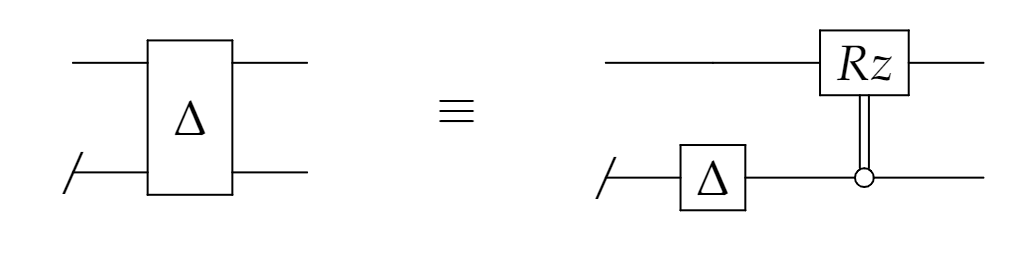
\includegraphics[scale=0.35]{img/QCircuit/diagonal/qcDelta.png}
	\caption{Decomposition of diagonal operators.} 
	\label{fig:shendeDiagDecomp}
\end{figure}
The next step is to find a way of decomposing the multiplexed gates such as the
$R_z$ gate presented above.\par

For the simple case of a singly-multiplexed $R_z$ gate, theorem 4 of
\cite{shendel06} provides a way of demultiplexing this operator, as shown in
figure \ref{fig:shendeSingleRz}.
\begin{figure}[!h]
	\centering
	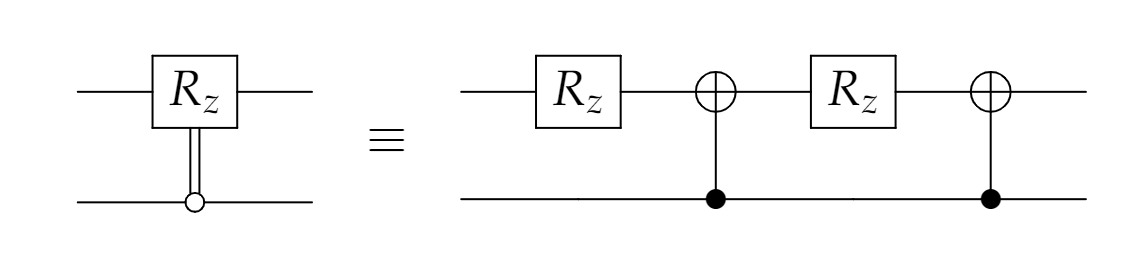
\includegraphics[scale=0.35]{img/QCircuit/diagonal/qcSingDecomp.png}
	\caption{Decomposition of a singly-multiplexed $R_z$ gate.} 
	\label{fig:shendeSingleRz}
\end{figure}
This can then be used to build the general case of the decomposition, as done
in theorem 8 of \cite{shendel06} and presented in figure
\ref{fig:shendeGeneralRz}. This method can be used to recursively decompose any
multiplexed rotation into basic gates, thus allowing the construction of a
circuit associated with any diagonal operator, depending on the choice of the
rotation angle.
\begin{figure}[!h]
	\centering
	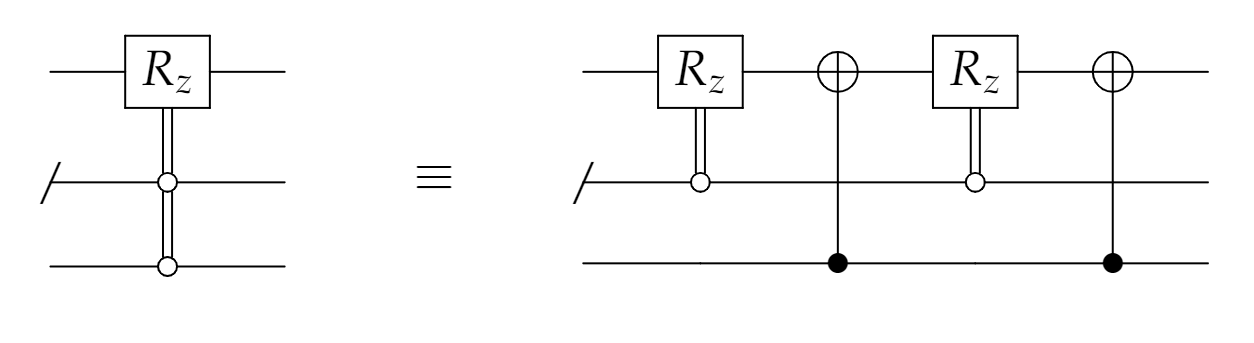
\includegraphics[scale=0.35]{img/QCircuit/diagonal/qcGenDecomp.png}
	\caption{General decomposition of a multiplexed $R_z$ gate.} 
	\label{fig:shendeGeneralRz}
\end{figure}\par

Finally, consider a simple multiplexor $R_z(\theta_0) \oplus R_z(\theta_1)$.
The choice of angle can be done as shown in figure
\ref{fig:shendeMultiplexorAngle}.

\begin{figure}[!h]
	\[  	\Qcircuit @C=1.5em @R=1.3em {
	               &   & \gate{R_z(\frac{\theta_0 + \theta_1}{2})} &\targ         & \gate{R_z(\frac{\theta_0 - \theta_1}{2})} & \targ    & \qw \\
                   &   & \qw        & \ctrl{-1}    &  \qw             & \ctrl{-1} & \qw
		          }\]
	\centering
	\caption{Choice of angle for a singly-multiplexed $R_z$ gate.}
	\label{fig:shendeMultiplexorAngle}
\end{figure}\par

With this background, consider the oracle operator for the Grover algorithm
performed on a circuit of $n=2$ qubits, for marked element $\ket{0}$. This
operator will be described by the following diagonal matrix
\begin{equation}
	\mathcal{O} = 
	\begin{pmatrix}
		-1 & 0 & 0 & 0 \\ 
		0 & 1 & 0 & 0 \\ 
		0 & 0 & 1 & 0 \\ 
		0 & 0 & 0 & 1 
	\end{pmatrix}.
\end{equation}
Its corresponding diagonal circuit is shown in figure \ref{fig:groverOracleCircuitQistkitDiagonal}.
\begin{figure}[!h]
        \centering
	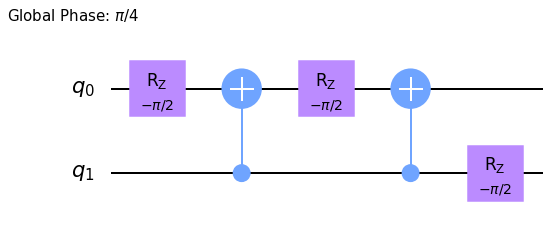
\includegraphics[scale=0.35]{img/Qiskit/GroverQiskit/Circuits/GroverQiskitCircOracle_N2_M0}
        \caption{Qiskit circuit of the  diagonal oracle operator for a search space of size  N=4  and marked element  \ket{m}=\ket{0} .}
        \label{fig:groverOracleCircuitQistkitDiagonal}
\end{figure}
The first two $R_z$ rotations correspond to the singly-multiplexed case, which
is decomposed as shown in figure \ref{fig:shendeSingleRz}. 

To understand the chosen angles, consider the list 
of phases associated with the diagonal entries of the oracle
\begin{equation} 
	[\alpha_0,\alpha_1,\alpha_2,\alpha_3] = [\pi,0,0,0].
\end{equation}\par
As was shown in figure \ref{fig:shendeMultiplexorAngle}, Qiskit will calculate $\theta_0$ and $\theta_1$ as
\begin{equation}
    [\theta_0, \theta_1] = [\alpha_1 - \alpha_0, \alpha_3 - \alpha_2] = [-\pi,0]
\end{equation}
which will result in the phase difference of $-\frac{\pi}{2}$. This will be applied recursively as in figure \ref{fig:shendeDiagDecomp}, and after the first iteration the vector will be modified to
\begin{equation}
        [\frac{\pi}{2},0,0,0]
\end{equation}
% Since two iterations were performed, the global phase will be calculated by 
% \begin{equation}
%     \varphi = (\frac{\alpha_0 + \alpha_1}{2} + \frac{\alpha_2 + \alpha_3}{2}) + \frac{\alpha_0 + \alpha_1}{2} = \frac{\pi + 0}{2} + \frac{0 + 0}{2} + \frac{\pi + 0}{2} = \frac{\pi}{4}
% \end{equation}
The rightmost $R_z$ rotation, represented by the $\Delta$ in the right side of figure \ref{fig:shendeDiagDecomp}, will contain the accumulated global phase and can be calculated by
\begin{equation}
e^{i\left(\frac{\pi}{4}\right)}R_z ()
\end{equation}
Applying the decomposition of the diagonal operators of figure \ref{}, 

\end{document}
